\documentclass{article}
\usepackage{graphicx}
\usepackage{color}
\usepackage{url}
\usepackage[font=small,labelfont=bf]{caption}
\usepackage[a4paper, total={16cm, 24cm}]{geometry}
\usepackage{indentfirst}



\begin{document}

\begin{titlepage}
    \begin{center}
        
	\begin{figure}
		\centering
        FACULTY OF MECHANICAL ENGINEERING AND ROBOTICS\\
        AGH UNIVERSITY OF SCIENCE AND TECHNOLOGY\\
        \vspace{0.2cm}
    	\begin{minipage}[b]{0.4\textwidth}
    	    \centering
    		\includegraphics[width=\textwidth]{IMG/AGH.png}
    	\end{minipage}
    	\hfill
    	\begin{minipage}[b]{0.4\textwidth}
	    	\centering
    		\includegraphics[width=\textwidth]{IMG/WIMIR.png}
		\end{minipage}
		\vspace{1cm}
    \end{figure}

    \Huge \textbf{Vision Controlled Mechanical Hand}
        
    \vspace{0.8cm}
    \LARGE 
    \color{black} 
            
    \vspace{0.8cm}       
    \textbf{Damian Durczok\\Mikolaj Gacek\\Adam Kolusz}        
    \vfill       
    \vspace{0.8cm}    
    12.03.2018
        
    \end{center}
\end{titlepage}

\tableofcontents
\break

\section{State of Art}
A typical mechatronic device encompasses many fields of technological engineering. This includes mechanical engineering, electronics, computer engineering, systems and control engineering.\\[12pt] 
\indent To thoroughly design such a system with awareness of all its elements during each step of the process requires the foresight and knowledge of all the components and relations between individual elements. This is the purpose of the state of art - a prerequisite to the initialization of a project. By the end of this section we will have explored existing technologies and solutions to our problem and drawn up a basic model of the mechatronic device.

\subsection{The Problem}
Certain situations that endanger human life benefit from the intervention of a robotic device. However, these robots may be limited in functionality compared to the human counterpart. In cases such as bomb disposal, nuclear power station decommissioning or handling of dangerous substances the dexterity of a human hand is significantly important.

\subsection{The Solution}
The mechanical hand is a device that has been iterated on many times in recent history. Control of such a hand is either by machine or human. For automated tasks, a machine controlled hand is more than sufficient. However, in unpredictable environments human intervention is still necessary.\\[12pt]
\indent This is where the idea stems together. A mechanical hand with the full dexterity of its real counterpart controlled in an intuitive way by a human. The control will be based on the idea of mimicking the operators limbs. Pairing this with a strategically placed camera and a virtual reality headset, we have an operator who is fully immersed and in full control of the situation at hand.

\subsection{Mechanical Hand}
Most modern innovations of the mechanical hand are related to the development of prosthetics. BeBionic \cite{bebionic} and Vincent Systems \cite{vincent} among many others have developed such devices that accurately mimic the likeness.

\begin{center}
\includegraphics[width=0.5\textwidth]{IMG/Bebionic_V2_Hand.png}
\captionof{figure}{BeBionic Mechanical Hand}
\end{center}

The most popular actuation method is a combination of a DC motor and either a worm gear or lead screw. The size of the hand leaves us with a very small working area, as a result the driving motors must be very small with high gear reductions.

\begin{center}
\includegraphics[width=0.6\textwidth]{IMG/fingerMech2.png}
\captionof{figure}{Mechanics of a finger \cite{JRRD}}
\end{center}

Another issue to contend with is the weight and speed of the mechanism. For prosthetic use, the hands are made to be lightweight for mobility. Whereas in our application this isn't a problem, we may still benefit from reducing the moments of inertia by increasing the acceleration capabilities of joints. Ideally having the same dynamic properties as the human hand.\\[12pt]
\indent The limited working space also forces certain optimization. For instance, not all joints need to be independently driven. We may simplify the model by involving mechanisms that create a fixed relationship between joints.

\begin{center}
\includegraphics[width=0.3\textwidth]{IMG/fingerMech.jpg}
\captionof{figure}{Reducing degrees of freedom mechanically \cite{JRRD}}
\end{center}

A final feature commonly observed is a certain flexion compliance level. Under a certain level of pressure, the joint flexes by either a spring or flexible material. This is a protective measure to prevent the damage of certain elements.\\[12pt]
\indent Many hobbyists opt out for a different solution that includes a motor and line. The joints are controlled in one direction by the contraction of a line and in the other by a spring or flexible material. This greatly simplifies the design process by allowing the motors to be located elsewhere. Potentially allowing for much larger drives and a greater gripping force along with greater movement speeds and accelerations. This system also naturally includes flexion compliance.

\begin{center}
\includegraphics[width=0.3\textwidth]{IMG/stringMech.jpg}
\captionof{figure}{Solidworks solution \cite{stringHand}}
\end{center}

This solution isn't as well researched as the earlier method and will require a longer prototyping faze. \\[12pt]
\indent Pneumatics may offer another solution. All the fingers are actuated by a pneumatic air muscle. These prove to have very high grip strength with favourable dynamic characteristics. All however comes with the price of size, to drive such a system a constant supply of compressed air is necessary to accurately position the stroke-length of each air muscle. Additionally a large valve system is necessary to control such a device.

\begin{center}
\includegraphics[width=0.4\textwidth]{IMG/airMuscle.jpg}
\captionof{figure}{Air Muscle}
\end{center}

In summary, we may consider driving our mechanism with either an electric motor or a pneumatic device. The pneumatic device may allow for much better dynamic performance such as limb velocity, acceleration and grip strength. However requires an entire pneumatic system in place which may prove expensive and resource heavy. The DC motor compromises on dynamic performance in place for a more ergonomic design.\\[12pt]
\indent The driving mechanism may be optimized by involving dependent joints. These joints may be driven directly or at a distance using lines. A line driven mechanism alleviates the problem of having to work in a small working area by removing the largest elements externally. 

\subsection{Sensors}
For the human hand to control the mechanical counterpart a set of sensors are necessary. For simplicity, we will only track the position of individual fingers. Although data sets such as grip strength, velocity or acceleration of fingers may inadvertently be natural features of some of the concepts.\\[12pt]
\indent A vision system introduces a non-invasive and non-contact method. Free to the public libraries such as OpenCV paired with a stereo camera system allow for creation of depth perception maps. After calibration of each camera and synchronization of frames, such a system will allow for accurate tracking.

\begin{center}
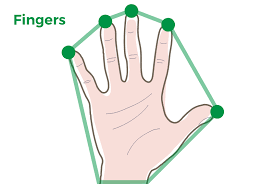
\includegraphics[width=0.5\textwidth]{IMG/HandSens.png}
\captionof{figure}{Visualization of hand recognition software}
\end{center}

\indent Microsoft released another interpretation of a motion sensing input design with the Xbox Kinect \cite{kinect}. The device includes an additional IR light source and an infrared camera for depth mapping and an RGB color VGA video camera for image recognition. The camera is capable of isolating the human from the background and with image recognition track individual limbs. The Microsoft SDK package for the system also includes access to the massive database for image recognition. This has been shown to work with small children using sign language learning software.\\[12pt]
\indent Plenty of other approaches also exist. One of the most popular is the usage of flex sensors. The concept is very simple, a change of resistance occurs with deflection, ie the flexing of a joint. The main disadvantage of such a solution is very low cost/efficiency ratio. However this method takes up very little space and low power consumption.\\[12pt] 
\indent Another accurate positioning method is with the use of multiple MPUs placed in carefully selected positions. If connected via a I2C protocol we may connect many along a single bus. These sensors are quite inexpensive compared to the flex sensor and provide acceptable accuracy when paired with suitable filters such as a Kalman filter. If not taken into account, the position obtained drifts over time resulting in a high error. However this can easily be mitigated.\\[12pt] 
\indent With a strategically placed camera and a line emitting IR blaster we may create a vision system that proves to be much more reliable than the previous concept. DIGITS \cite{Digits} is the realization of such a device. It is capable of emulating the human hand in a virtual environment with great success.

\begin{center}
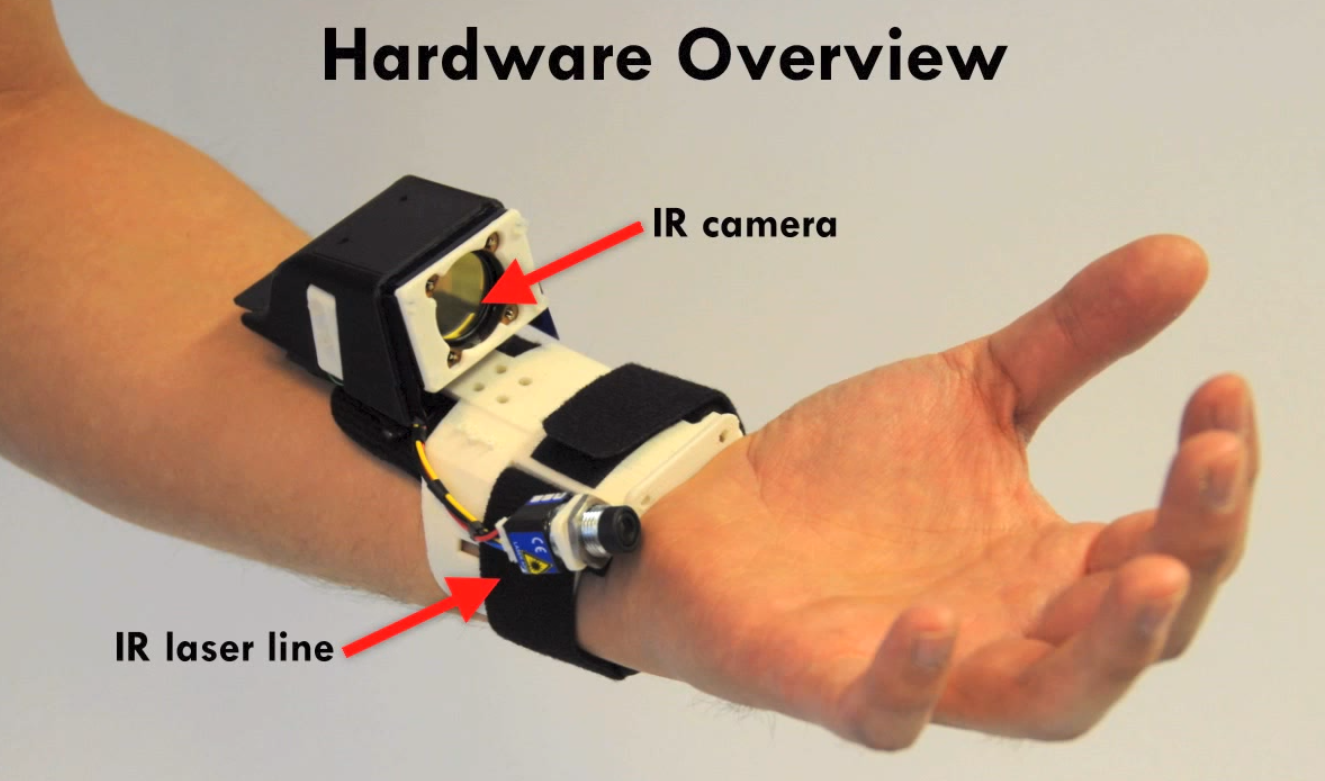
\includegraphics[width=0.5\textwidth]{IMG/HandSens02.png}
\captionof{figure}{A finger position method by Digits \cite{Digits}}
\end{center}

\indent The IR blaster greatly increases the image recognition performance by giving it obvious vision cues. The wrist mounted device may also benefit from an additional MPU sensor that will provide us with information on the placement of the arm. Such a system is not limited by the environment; lighting levels and surrounding colors wouldn't have a significant impact on the performance of the mechanism.

\subsection{Control}

For an electronic control system we may consider two distinct architectures that will be ideal for our device; an FPGA board or a microcomputer like the Raspberry Pi. Both devices are capable of image signal processing with the use of the OpenCV library, therefore all techniques discussed above are viable. In extension, OpenCL (an official and supported extension to OpenCV) can be used inplace of HDL in FPGA to improve design productivity. The main advantage of FPGA over a CPU is parallelism\cite{FPGA}. In a system where many sensors and actuators are present, and a quick response of a mechanical hand is essential this can become a major advantage over traditional microcomputers. However, this comes with a cost of complexity.\\[12pt]
\indent Both systems are also capable of signal filtering and noise reduction. This can reduce micro motions and sensor imperfections to create a much more fluid movement of the hand. Additionally, machine learning could incorporate a decision making process that could create precise maneuvers even if the operator isn't fully trained or capable of them.  Potentially becoming an enhanced extension of the human by providing stability and limiting the motion to avoid accidental jerks or unwanted reflexes.

\section{Concept}
\subsection{Mechanics}

The primary attributes of our mechanical hand will be its gripping capabilities and precision. To achieve this while keeping the entire project within acceptable dimensions we need to introduce dependent joints with certain flexion compliance. \\[12pt] 
\indent Some of the dependent joints will have an additional mechanism extended from it. This mechanism will usually consist of a spring that is pushing on a lever. With no external forces, the lever will be sitting in a locked maximum position. The moment it comes into contact with something and depending on the amount of force applied, the lever hinges back. This gives the dependent joint a certain amount of restricted movement that mimics the joints of the hand in a similar fashion. This sort of compliance will greatly increase the hands holding capabilities by being able to mechanically adapt to the objects geometrical features. \\[12pt]
\indent A single hand will be comprised of three digits, each with two degrees of controlled motion. However, due to flexion compliance it will have many more degrees of freedom. The human hand has four bones for each finger and three for the thumb. The bones go as follows from the tip of the finger to the wrist; distal phalanges, medial phalanges, proximal phalanges and the metacarpals. With the thumb lacking the medial phalanges. Each finger has four degrees of freedom except for the thumb by only having three. Next we will explore all our joints and describe how we plan to resolve them. \\[12pt]
\indent The first is the opposable thumb, which will have two joints and one degree of controlled motion. The distal phalanges will have flexion compliance, while the metacarpal will be driven by a larger motor to match the cumulative force of the other joints. The thumb needs to be as universal as its counterpart. Both grip strength and precision tasks paired with the other fingers are important. \\[12pt]
\indent The index finger will have four joints and also two degrees of motion. The distal phalanges will have 90 degree flexion compliance and is dependent on the angle of the medial phalanges. The medial phalanges and proximal phalanges will be each driven by a motor, while the metacarpals will be attached by ball joint and given minimal flexion compliance. \\[12pt]
\indent The final three fingers will be combined into one larger finger. Since these fingers are usually used for gripping and handling of objects, they will be mounted with larger motors and the larger surface area will provide a better gripping surface. The joint mobility will be similar to the index finger. \\[12pt]
\indent The last area to cover is the palm. The metacarpals is responsibly for its shape. We have two metacarpals that have flexion compliance and one on the thumb that is driven. This means the palm has the capability of adjusting its shape to a gripped object.

\subsection{Control and Sensors}

With the mechanical end of the project providing advantages gripping mechanisms and variable grip strength, the control of the device may be much more forgiving and the use of haptic feedback isn't as necessary. With this in mind, we may create a completely non invasive human operated controller with the use of vision systems. \\[12pt]
\indent The system will be made up of two cameras that will provide stereo vision. With proper calibration, we may produce a depth map and isolate a human operator from the background. Once isolated, it is a matter of manipulating the image and developing algorithms that may track geometrical features. Libraries such as OpenCV already provide most of these features in languages such as Python and C++. \\[12pt]
\indent The readings from the camera may be further improved by adding a layer of machine decision making. Certain filters for noise reduction are certainly necessary, however we may also include pre-programmed operations that may assist the human and become an extension of him. For instance, we may limit the velocity of fingers to reduce abrupt movements in certain situations or remember the gripping position for a certain object. This way the operator carries out the general movement required of the robot and the robot decides on the precise movements that may be difficult for the user to control. 

\subsection{Electronics and Actuating}

Since the image signals from two cameras have to be processed in real-time it is important to consider a capable computer. We decided that the entire Vision System will be run on Raspberry Pi 3 Model B microcomputer. This device possesses a quad-core 64bit processor and 1GB RAM, hence is capable of performing desired operations. Further reassurance of its capabilities is the many camera modules and OpenCV projects already developed for the Raspberry.\\[12pt]
\indent The robotic fingers will be actuated by six servomotors controlled by an Arduino Uno R3 attached to the hand. The Arduino Uno R3 has 14 digital input/output pins (of which 6 can be used as PWM outputs). The wireless connection between the Raspberry Pi 3 B and the Arduino will be implemented with the use of a Bluetooth protocol. The Raspberry has a built-in Bluetooth module and Arduino can be easily extended with a HC-0x series Bluetooth module.\\[12pt] 
\indent	The Arduino controller and motors will be energized by an individual power supply with a voltage stabilizer. The Raspberry Pi will be energized by a set of 18650 cells through a voltage stabilizer.










\break
\begin{thebibliography}{1}
	\bibitem{bebionic} BeBionic. Retrieved from {\url{http://bebionic.com/the_hand/technical_information/}} 
	\bibitem{vincent} VincentSystems. Retrieved from {\url{  https://vincentsystems.de/en/}} 
	\bibitem{JRRD} U.S. Department of Veterans Affairs, {\em Journal of Rehabilitation Research And Development}. Volume 50 Number 5, 2013
   Pages 599-618 Retrieved form {\url{https://www.rehab.research.va.gov/jour/2013/505/page599.html}}
	\bibitem{stringHand} SOLIDWORKS. Retrieved from {\url{ http://blogs.solidworks.com/tech/2016/08/solidworks-time-lapse-tutorial-mechanical-hand.html}}
	\bibitem{airMuscle} Peter Scarfe, Euan Lindsay {\em Air Muscle Actuated Low Cost Humanoid Hand}. Retrieved from {\url{ http://cdn.intechopen.com/pdfs/4176/InTech-Air_muscle_actuated_low_cost_humanoid_hand.pdf
}} 
	\bibitem{kinect} Kinect. Retrieved from {\url{https://www.jameco.com/jameco/workshop/howitworks/xboxkinect.html}}
	\bibitem{Digits} DIGITS. Retrieved from {\url{https://spectrum.ieee.org/video/consumer-electronics/audiovideo/digits-hands-free-3d}}	
	\bibitem{ALTERA} Altera, Video and Image Processing Design Using FPGAs. Retrieved from {\url{https://www.altera.com/en_US/pdfs/literature/wp/wp-video0306.pdf}}
	\bibitem{CpuFpga} Brandon Treece ,VisionSystems Design. Retrieved from {\url{https://www.vision-systems.com/articles/print/volume-22/issue-8/features/cpu-or-fpga-for-image-processing-which-is-best.html	}}
	\bibitem{FPGA} FPGA in Robotics. Retrieved from {\url{https://robotics.stackexchange.com/questions/1153/when-should-fpgas-be-used-in-robotics}}
	\bibitem{CpuFpga02} APUs vs FPGAs. Retrieved from {\url{http://www.electronicdesign.com/microprocessors/apus-vs-fpgas-battle-smart-camera-processing-supremacy}}
	\bibitem{Intel} Intel FPGA SDK for OpenCL. Retrieved from {\url{https://www.altera.com/en_US/pdfs/literature/hb/opencl-sdk/aocl_programming_guide.pdf}}
	\bibitem{OpenCL} OpenCL. Retrieved from {\url{https://opencv.org/platforms/opencl.html}}
	\bibitem{VisionProcessing} Video and Image Processing Suite Intel FPGA IP. Retrieved from {\url{https://www.altera.com/products/intellectual-property/ip/dsp/m-alt-vipsuite.html}}
	\bibitem{Grip} A comparison of the grip force distribution in natural hands and in prosthetic hands. Retrieved from {\url{https://pdfs.semanticscholar.org/f600/c0ad7d6ecb7510b1b8e8f1318ffa03bb48cd.pdf}}



\end{thebibliography}
  
\end{document}